Dưới đây là mô tả chi tiết các entity, nêu ra vai trò, attribute và các relationship trong hệ thống.

\begin{figure}[H]
  \centering
  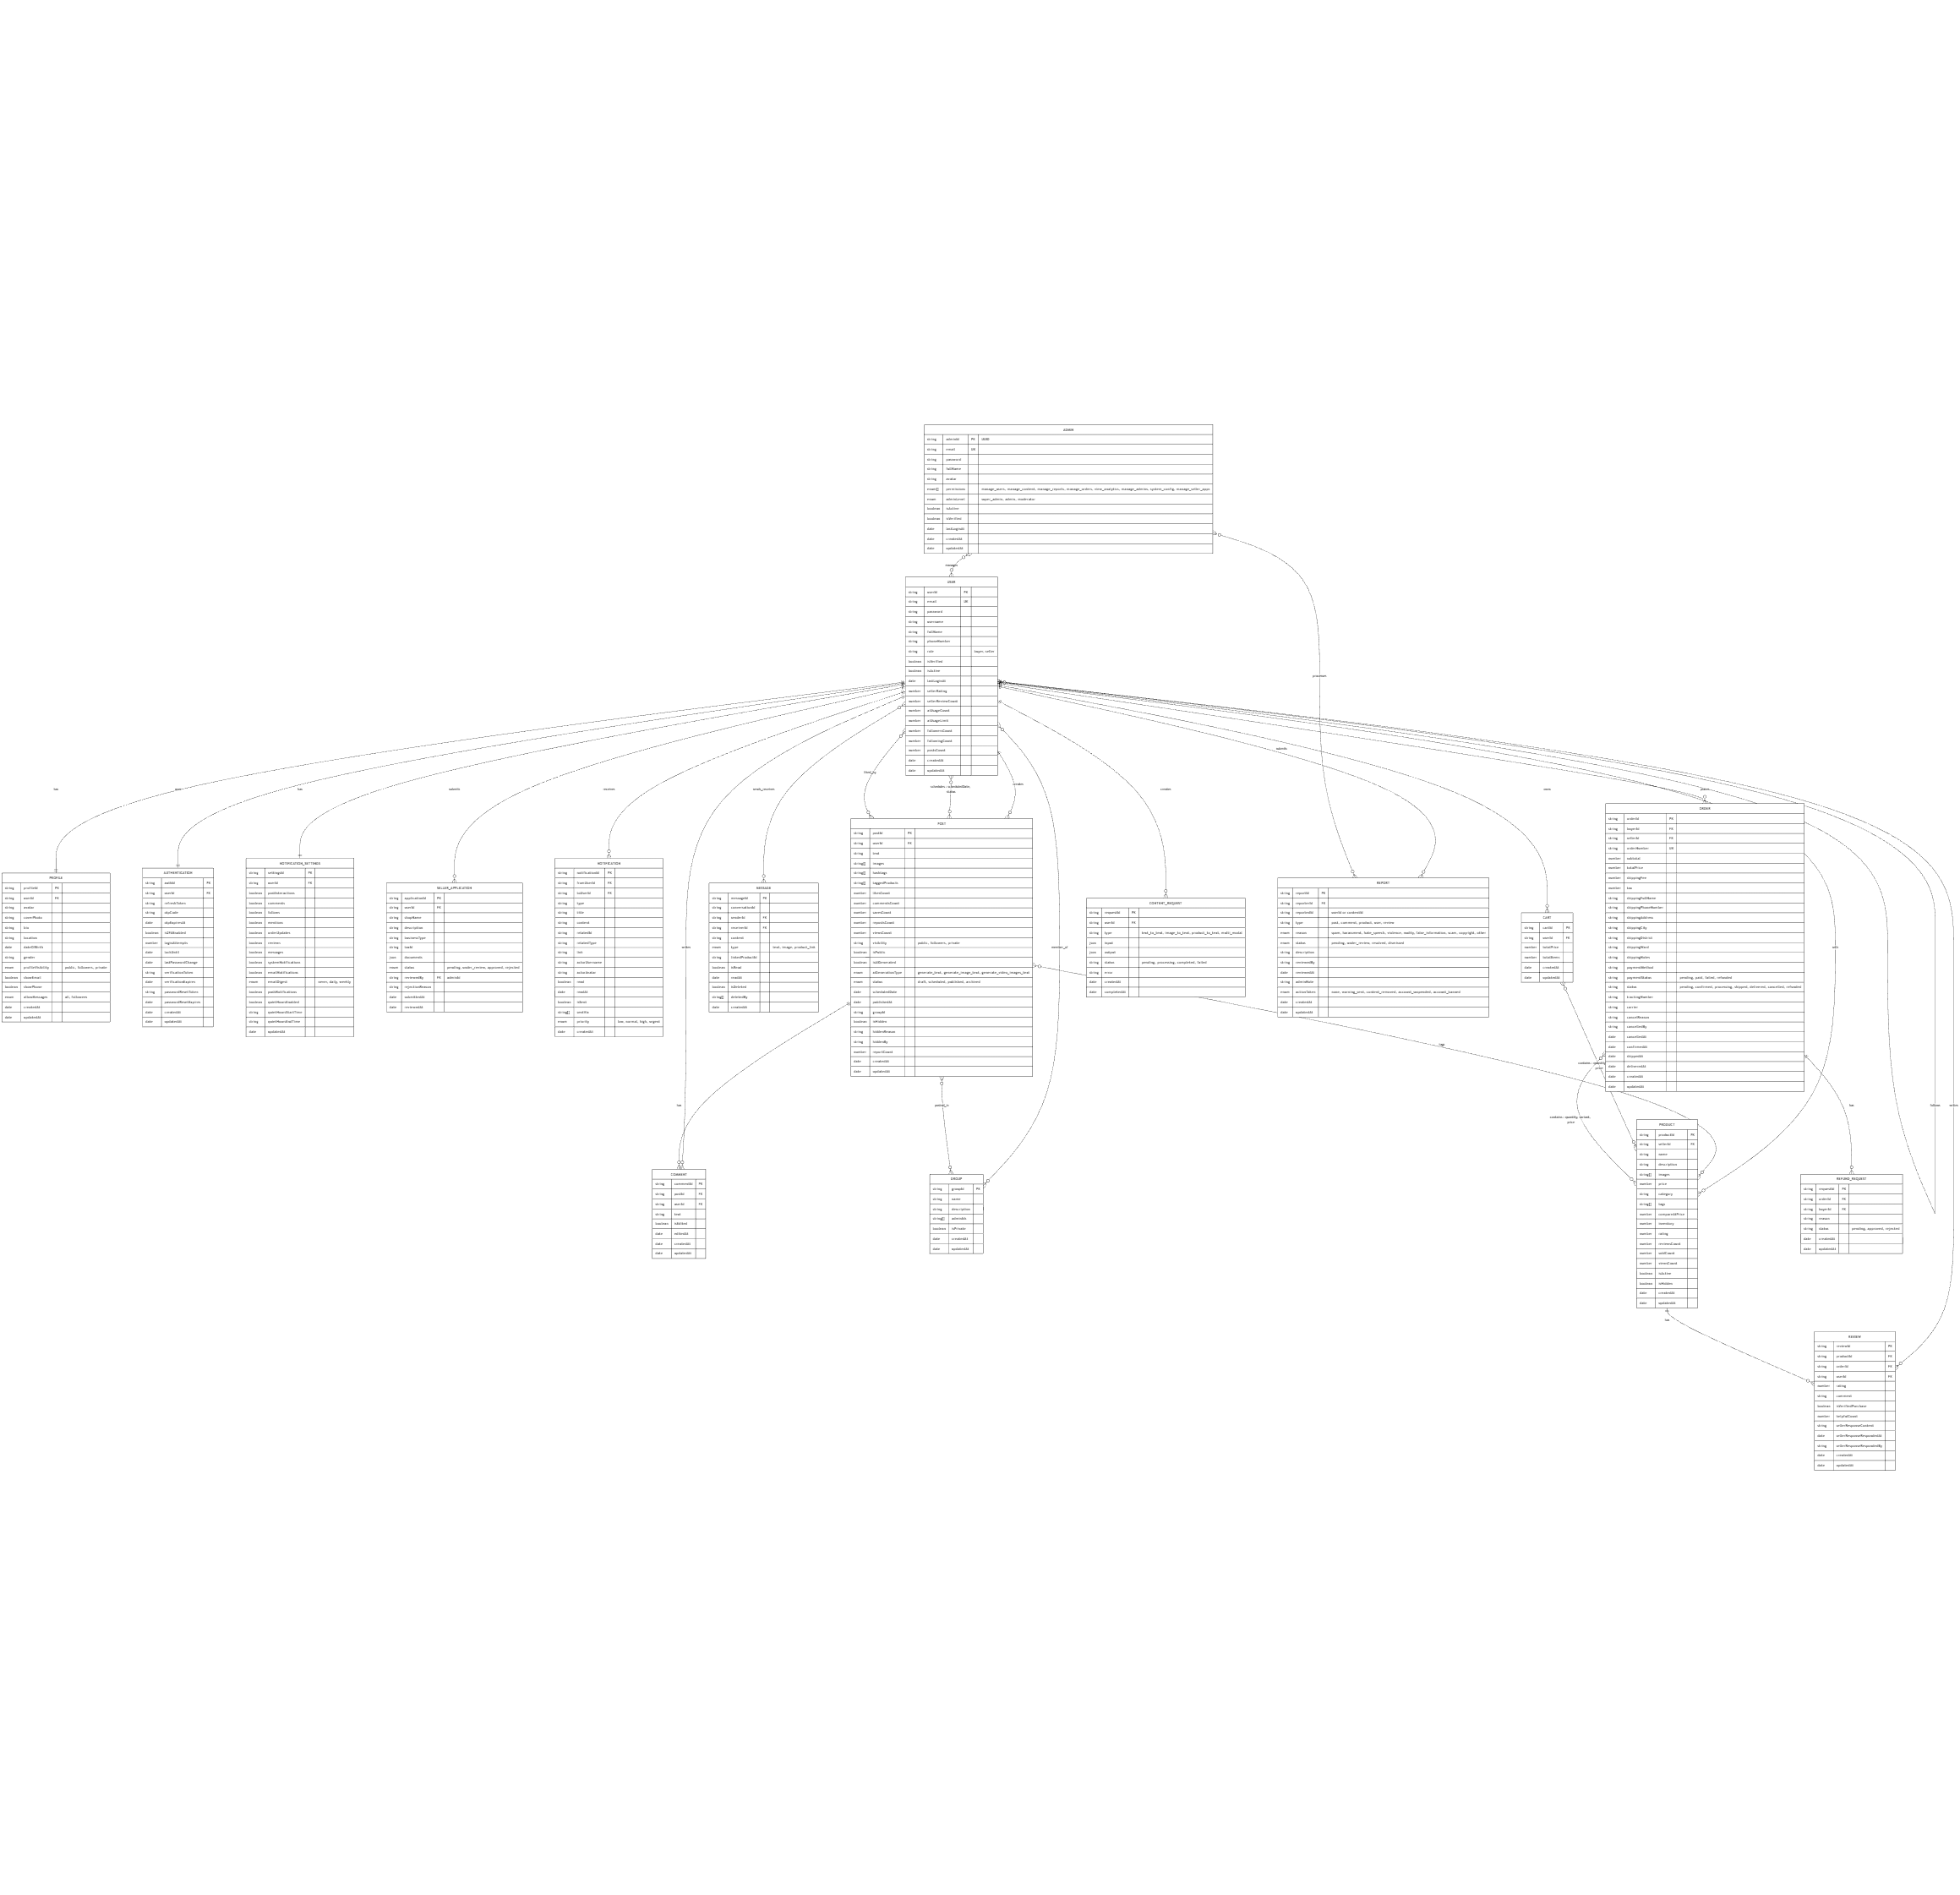
\includegraphics[width=\textwidth]{Images/ERD.png}
  \caption{Sơ đồ ERD (Entity Relationship Diagram) - Mô hình thực thể kết hợp của hệ thống}
  \label{fig:erd-diagram}
\end{figure}

\subsection{Thực thể (Entities)}
\paragraph{USER} Entity đại diện cho người dùng chung của hệ thống (buyer hoặc seller). Attributes: \textit{userId} (PK), email (UK), password, username, fullName, role (buyer/seller), isVerified, isActive, aiUsageCount (số lần đã sử dụng AI), aiUsageLimit (giới hạn số lần sử dụng AI), followersCount, followingCount, (...), createdAt, updatedAt.

\paragraph{PROFILE} Entity lưu trữ hồ sơ công khai/riêng tư gắn với người dùng. Attributes: \textit{profileId} (PK), \textit{userId} (FK), avatar, coverPhoto, bio, location, profileVisibility (public/followers/private), showEmail, allowMessages (all/followees), (...), createdAt, updatedAt.

\paragraph{AUTHENTICATION} Entity quản lý thông tin đăng nhập và bảo mật. Attributes: \textit{authId} (PK), \textit{userId} (FK), refreshToken, otpCode, otpExpiresAt, is2FAEnabled, loginAttempts, lockUntil, verificationToken, passwordResetToken, (...), createdAt, updatedAt.

\paragraph{NOTIFICATION\_SETTINGS} Entity lưu trữ cấu hình thông báo cá nhân. Attributes: \textit{settingsId} (PK), \textit{userId} (FK), postInteractions, comments, follows, orderUpdates, reviews, messages, emailNotifications, emailDigest (never/daily/weekly), pushNotifications, quietHoursEnabled, (...), updatedAt.

\paragraph{NOTIFICATION} Entity lưu trữ bản ghi thông báo gửi tới người dùng. Attributes: \textit{notificationId} (PK), fromUserId (FK), toUserId (FK), type, title, content, relatedId, relatedType, link, read, readAt, priority (low/normal/high/urgent), (...), createdAt.

\paragraph{POST} Entity đại diện cho bài viết của người dùng. Attributes: \textit{postId} (PK), \textit{userId} (FK), text (nội dung văn bản), images[] (danh sách ảnh), hashtags[], taggedProducts[], likesCount, commentsCount, viewsCount, visibility (public/followers/private), isAIGenerated (được tạo bởi AI), aiGenerationType (generate\_text/generate\_image\_text/generate\_video\_images\_text - loại tạo nội dung AI), status (draft/scheduled/published/archived), scheduledDate, publishedAt, (...), createdAt, updatedAt.

\paragraph{COMMENT} Entity đại diện cho bình luận trên bài viết. Attributes: \textit{commentId} (PK), \textit{postId} (FK), \textit{userId} (FK), text, isEdited, editedAt, createdAt, updatedAt.

\paragraph{GROUP} Entity đại diện cho nhóm cộng đồng. Attributes: \textit{groupId} (PK), name, description, adminIds[], isPrivate, createdAt, updatedAt.

\paragraph{MESSAGE} Entity lưu trữ tin nhắn giữa người dùng. Attributes: \textit{messageId} (PK), conversationId, senderId (FK), receiverId (FK), content, type (text/image/product\_link), linkedProductId, isRead, readAt, (...), createdAt.

\paragraph{PRODUCT} Entity đại diện cho sản phẩm do người bán đăng. Attributes: \textit{productId} (PK), sellerId (FK), name, description, images[], price, category, tags[], compareAtPrice, inventory, rating, reviewsCount, soldCount, viewsCount, isActive, (...), createdAt, updatedAt.

\paragraph{CART} Entity đại diện cho giỏ hàng của người mua. Attributes: \textit{cartId} (PK), \textit{userId} (FK), totalPrice, totalItems, createdAt, updatedAt.

\paragraph{ORDER} Entity đại diện cho đơn hàng giữa người mua và người bán. Attributes: \textit{orderId} (PK), buyerId (FK), sellerId (FK), orderNumber (UK), subtotal, totalPrice, shippingFee, shippingAddress, shippingCity, paymentMethod, paymentStatus (pending/paid/failed/refunded), status (pending/confirmed/processing/shipped/delivered/cancelled/refunded), trackingNumber, refund\_status, refund\_reason, (...), createdAt, updatedAt.

\paragraph{REVIEW} Entity đại diện cho đánh giá sản phẩm gắn với đơn. Attributes: \textit{reviewId} (PK), productId (FK), orderId (FK), userId (FK), rating, comment, isVerifiedPurchase, helpfulCount, sellerResponseContent, (...), createdAt, updatedAt.

\paragraph{REFUND\_REQUEST} Entity đại diện cho yêu cầu hoàn tiền cho đơn. \textbf{Lưu ý:} Trong schema thực tế, các trường refund được tích hợp vào bảng \textit{orders} (refund\_status, refund\_reason, refund\_requested\_at, refund\_processed\_at, refund\_processed\_by).

\paragraph{CONTENT\_REQUEST} Entity lưu trữ yêu cầu tạo nội dung AI. Attributes: \textit{requestId} (PK), userId (FK), type (generate\_text/generate\_image\_text/generate\_video\_images\_text - loại yêu cầu), input (json - dữ liệu đầu vào), output (json - kết quả đầu ra), status (pending/processing/completed/failed), error, createdAt, completedAt.

\paragraph{REPORT} Entity lưu trữ báo cáo vi phạm. Attributes: \textit{reportId} (PK), reporterId (FK), reportedId, type (post/comment/product/user/review), reason (spam/harassment/hate\_speech/violence/nudity/false\_information/scam/copyright/other), status (pending/under\_review/resolved/dismissed), description, reviewedBy, actionTaken (none/warning\_sent/content\_removed/account\_suspended/account\_banned), (...), createdAt, updatedAt.

\paragraph{SELLER\_APPLICATION} Entity lưu trữ hồ sơ đăng ký trở thành người bán. Attributes: \textit{applicationId} (PK), userId (FK), shopName, description, businessType, taxId, documents (json), status (pending/under\_review/approved/rejected), reviewedBy, rejectionReason, submittedAt, reviewedAt.

\paragraph{ADMIN} Entity đại diện cho tài khoản quản trị. Attributes: \textit{adminId} (PK, UUID), email (UK), password, fullName, avatar, permissions[] (manage\_users/manage\_content/manage\_reports/manage\_orders/view\_analytics/manage\_admins/system\_config/manage\_seller\_apps), adminLevel (super\_admin/admin/moderator), isActive, isVerified, lastLoginAt, createdAt, updatedAt.

\subsection{Mối quan hệ (Relationships)}
\begin{itemize}
  \item \textbf{USER -- PROFILE}: 1:1. Mỗi USER có đúng một PROFILE; mỗi PROFILE chỉ thuộc một USER.
  \item \textbf{USER -- AUTHENTICATION}: 1:1. Lưu token/OTP và cấu hình 2FA cho đúng một USER.
  \item \textbf{USER -- NOTIFICATION\_SETTINGS}: 1:1. Mỗi USER có cấu hình thông báo riêng.
  \item \textbf{USER -- NOTIFICATION}: 1:N. Một USER nhận nhiều thông báo qua toUserId; fromUserId ghi nhận tác nhân phát sinh.
  \item \textbf{USER -- SELLER\_APPLICATION}: 1:N. Người dùng có thể nộp nhiều đơn đăng ký bán.
  \item \textbf{ADMIN -- USER}: N:M (quản lý). ADMIN có thể quản lý nhiều USER và ngược lại (phân ca/phạm vi).
  \item \textbf{USER -- USER (follow)}: N:M. Người dùng có thể theo dõi lẫn nhau.
  \item \textbf{POST -- COMMENT}: 1:N. Một POST có nhiều COMMENT; COMMENT thuộc duy nhất một POST.
  \item \textbf{USER -- POST}: 1:N. Người dùng tạo nhiều POST; mỗi POST thuộc một USER.
  \item \textbf{USER -- COMMENT}: 1:N. Người dùng viết nhiều COMMENT.
  \item \textbf{POST -- USER (liked\_by)}: N:M. Một bài có nhiều người thích; một người thích nhiều bài.
  \item \textbf{POST -- GROUP (posted\_in)}: N:M. Bài viết có thể được đăng trong nhiều GROUP; GROUP chứa nhiều bài.
  \item \textbf{POST -- PRODUCT (tags)}: N:M. Bài viết có thể gắn nhiều sản phẩm; sản phẩm có thể được tag ở nhiều bài.
  \item \textbf{USER -- GROUP (member\_of)}: N:M. Người dùng có thể tham gia nhiều nhóm; nhóm có nhiều thành viên.
  \item \textbf{USER -- MESSAGE}: N:M. Một USER gửi/nhận nhiều MESSAGE; mỗi MESSAGE có sender và receiver.
  \item \textbf{USER -- POST (schedules)}: N:M qua thuộc tính scheduling. Một USER có thể lên lịch nhiều POST; một POST có thể có bản ghi lịch.
  \item \textbf{USER -- PRODUCT}: 1:N. Một người bán đăng nhiều PRODUCT; mỗi PRODUCT thuộc một seller.
  \item \textbf{CART -- PRODUCT}: N:M. Một CART chứa nhiều PRODUCT (kèm quantity/variant/price trên dòng giỏ); một PRODUCT có thể nằm trong nhiều CART.
  \item \textbf{ORDER -- PRODUCT}: N:M. Một ORDER chứa nhiều PRODUCT (dòng hàng gồm quantity/variant/price); một PRODUCT xuất hiện trong nhiều ORDER.
  \item \textbf{USER -- CART}: 1:N (thiết kế cho phép nhiều giỏ theo phiên; thực tế thường 1). Mỗi CART thuộc một USER.
  \item \textbf{USER -- ORDER}: 1:N. Người mua có nhiều ORDER; mỗi ORDER gắn với một buyer. Đồng thời ORDER giữ sellerId để biết người bán.
  \item \textbf{USER -- REVIEW}: 1:N. Người dùng viết nhiều REVIEW.
  \item \textbf{PRODUCT -- REVIEW}: 1:N. Một PRODUCT có nhiều REVIEW.
  \item \textbf{ORDER -- REFUND\_REQUEST}: 1:N. Một ORDER có thể phát sinh nhiều REFUND\_REQUEST.
  \item \textbf{USER -- REFUND\_REQUEST}: 1:N. Người mua gửi nhiều yêu cầu hoàn.
  \item \textbf{USER -- CONTENT\_REQUEST}: 1:N. Người dùng tạo nhiều yêu cầu AI; mỗi yêu cầu thuộc một USER.
  \item \textbf{USER -- REPORT}: 1:N. Người dùng có thể gửi nhiều REPORT; mỗi REPORT có một reporter.
  \item \textbf{ADMIN -- REPORT}: N:M. Nhiều ADMIN có thể xử lý các REPORT, mỗi REPORT có thể được giao/lưu vết nhiều admin.
\end{itemize}

\subsection{Chuyển đổi từ ERD sang Database Schema}

Quá trình chuyển đổi từ mô hình ERD sang database schema PostgreSQL đã được thực hiện với các quyết định thiết kế cụ thể để tối ưu performance, đảm bảo data integrity và hỗ trợ các tính năng của hệ thống.

\subsubsection{Quyết định về cấu trúc bảng (Table Structure)}

\paragraph{Junction Tables cho quan hệ N:M}
Để hỗ trợ các relationship N:M, hệ thống đã tách thành các junction table riêng biệt thay vì sử dụng array:

\begin{itemize}
  \item \textbf{post\_likes}: Lưu trữ relationship giữa POST và USER (liked\_by). Mỗi record gồm post\_id, user\_id và created\_at. Có UNIQUE constraint (post\_id, user\_id) để đảm bảo một người dùng chỉ like một bài viết một lần.
  \item \textbf{post\_saves}: Tương tự cho chức năng lưu bài viết (bookmark).
  \item \textbf{post\_reposts}: Lưu trữ các bài viết được chia sẻ lại (repost).
  \item \textbf{review\_helpful\_votes}: Lưu trữ các vote "hữu ích" cho đánh giá sản phẩm.
  \item \textbf{group\_members}: Quản lý thành viên của nhóm với role (member/admin/moderator), thay vì chỉ dùng adminIds[] trong GROUP.
  \item \textbf{user\_follows}: Relationship follow giữa người dùng với UNIQUE constraint (follower\_id, following\_id) và CHECK constraint để tránh tự follow.
  \item \textbf{user\_blocks}: Relationship block giữa người dùng (không có trong ERD nhưng cần thiết cho tính năng chặn người dùng).
\end{itemize}

\paragraph{Denormalization}
Một số quyết định gộp bảng để tối ưu query performance:

\begin{itemize}
  \item \textbf{REFUND\_REQUEST → orders}: Thay vì tạo bảng REFUND\_REQUEST riêng như trong ERD, các trường refund được tích hợp trực tiếp vào bảng \textit{orders}:
  \begin{itemize}
    \item refund\_requested (BOOLEAN)
    \item refund\_status (pending/approved/rejected)
    \item refund\_reason (TEXT)
    \item refund\_requested\_at, refund\_processed\_at (TIMESTAMP)
    \item refund\_processed\_by (FK → users)
  \end{itemize}
  Lý do: Mỗi đơn hàng chỉ có tối đa một yêu cầu hoàn tiền, việc gộp giảm số lượng JOIN và tăng query performance.
\end{itemize}

\paragraph{Supporting Tables}
Các bảng hỗ trợ được tách để quản lý metadata và lịch sử:

\begin{itemize}
  \item \textbf{product\_images}: Tách từ images[] trong PRODUCT để lưu metadata (url, public\_id, is\_primary, width, height) và hỗ trợ quản lý ảnh tốt hơn.
  \item \textbf{post\_images}: Tương tự cho POST (mặc dù posts vẫn giữ images[] để backward compatibility).
  \item \textbf{review\_images}: Ảnh đính kèm trong đánh giá sản phẩm.
  \item \textbf{report\_screenshots}: Ảnh chụp màn hình trong báo cáo vi phạm.
  \item \textbf{order\_status\_history}: Lưu lịch sử thay đổi trạng thái đơn hàng với timestamp, note và updated\_by để audit trail.
  \item \textbf{product\_variants} và \textbf{product\_variant\_options}: Hỗ trợ biến thể sản phẩm (size, color, etc.) với giá và tồn kho riêng.
\end{itemize}

\subsubsection{Sơ đồ Relational Mapping}
Hình \ref{fig:relational-mapping} mô tả sơ đồ relational mapping của hệ thống, thể hiện tất cả các bảng và mối quan hệ giữa chúng thông qua Primary Keys (PK) và Foreign Keys (FK). Sơ đồ này được tạo từ database schema PostgreSQL thực tế, bao gồm các junction tables cho quan hệ N:M và các supporting tables đã được mô tả ở trên.

\begin{figure}[H]
  \centering
  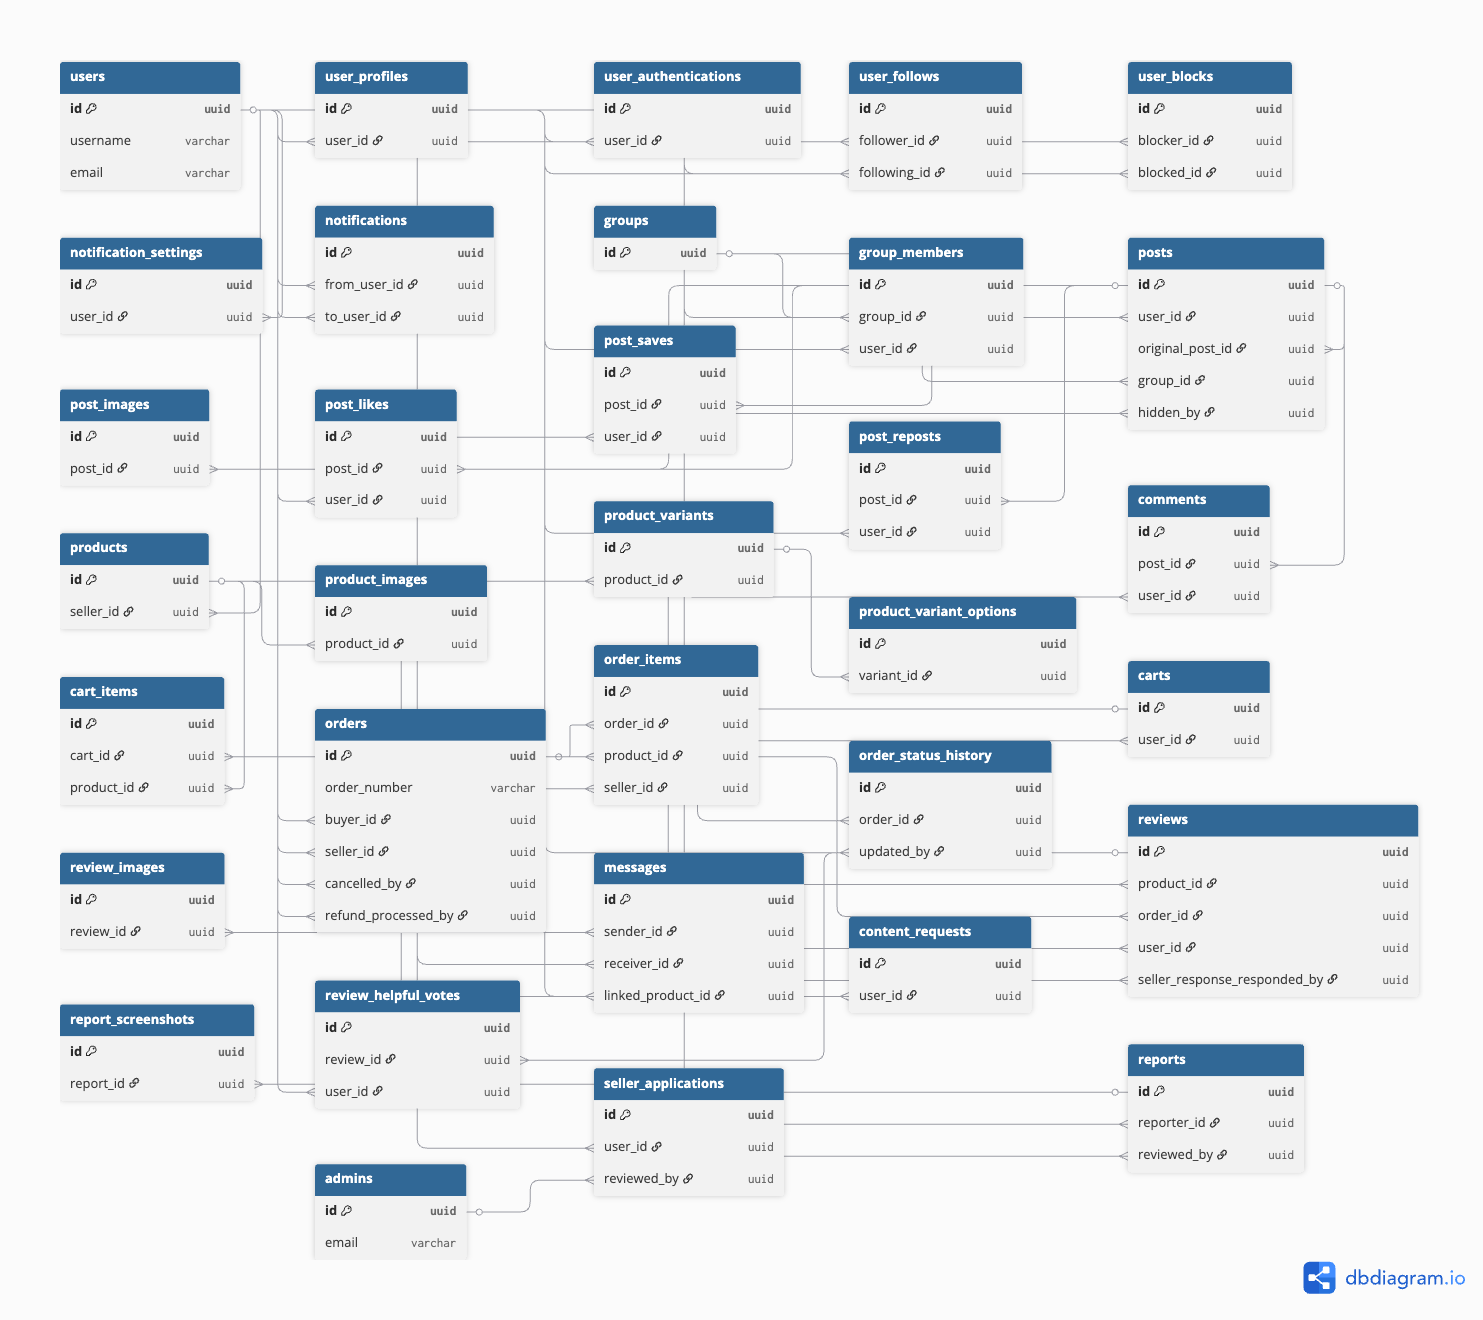
\includegraphics[width=\textwidth]{Images/Relation-Mapping.png}
  \caption{Sơ đồ Relational Mapping - Các bảng và mối quan hệ trong database schema}
  \label{fig:relational-mapping}
\end{figure}
